
\chapter[Bài tập: Thay đổi chiều dài và gia tốc trọng trường trong các bài toán về con lắc đơn;\\Dạng bài: Năng lượng của con lắc đơn]{Bài tập: Thay đổi chiều dài và gia tốc trọng trường\\ trong các bài toán về con lắc đơn;\\Dạng bài: Năng lượng của con lắc đơn}
\section{Lý thuyết}
\subsection{Chu kỳ của con lắc vướng đinh}
Một dao động toàn phần của con lắc bị vướng đinh gồm 2 giai đoạn:
\begin{itemize}
	\item Giai đoạn 1: Con lắc dao động với chiều dài $l_1$ và chu kỳ $T_1$:
	\begin{equation*}
		T_1=2\pi \sqrt{\dfrac{l_1}{g}}.
	\end{equation*} 
	\item Giai đoạn 2: Con lắc dao động với chiều dài $l_2$ và chu kỳ $T_2$:
	\begin{equation*}
		T_2=2\pi \sqrt{\dfrac{l_2}{g}}.
	\end{equation*}  
	\item Chu kỳ của con lắc vướng đinh:
	\begin{equation*}
		T=\dfrac{1}{2}T_1 +\dfrac{1}{2}T_2 = \dfrac{1}{2} (T_1 + T_2).
	\end{equation*}
	\begin{center}
		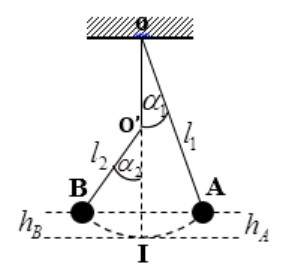
\includegraphics{../figs/VN12-PH-04-A-003-4-V2-1.JPG}
	\end{center}
	\luuy{Nếu con lắc vướng đinh ở vị trí khác, ta cần phải xác định được thời gian con lắc chuyển động với chiều dài $l$ và thời gian chuyển động với chiều dài $l'$ trong một chu kì.}
\end{itemize}
\subsection{Chu kỳ con lắc đơn khi thay đổi nhiệt độ và độ cao}
\subsubsection{Thay đổi nhiệt độ}
\begin{itemize}
	\item Ở nhiệt độ $t_1$: 
	\begin{equation*}
		T_1=2\pi\sqrt{\dfrac{l_1}{g}},
	\end{equation*}
	với $l_1=l_0 (1+\alpha t_1)$.
	\item Ở nhiệt độ $t_2$: 
	\begin{equation*}
		T_1=2\pi\sqrt{\dfrac{l_2}{g}},
	\end{equation*}
	với $l_2=l_0 (1+\alpha t_2)$.
	\item Lập tỉ số $T_1$ và $T_2$, suy ra:
	\begin{equation*}
		\dfrac{\Delta T}{T_1} = \dfrac{T_2-T_1}{T_1} =\dfrac{1}{2} \alpha (t_2 -t_1).
	\end{equation*}
\end{itemize}
\subsubsection{Thay đổi độ cao}
\begin{itemize}
	\item Ở mặt đất:
	\begin{equation*}
		T=2\pi \sqrt{\dfrac{l}{g}},
	\end{equation*}
	với $g = G \dfrac{M}{R^2}$.
	\item Ở độ cao $h$:
	\begin{equation*}
		T'=2\pi \sqrt{\dfrac{l}{g'}}, 
	\end{equation*}
	với $g'= G \dfrac{M}{(R+h)^2}$.
	\item Lập tỉ số $T'$ và $T$, suy ra: 
	\begin{equation*}
		\dfrac{\Delta T}{T} = \dfrac{T'-T}{T} =\dfrac{h}{R}.
	\end{equation*}
\end{itemize}
\subsubsection{Thay đổi cả độ cao và nhiệt độ}

\begin{equation*}
	\dfrac{\Delta T}{T}=\dfrac{h}{R} +\dfrac{1}{2} \alpha (t_2-t_1).
\end{equation*}
\subsection{Sự nhanh (chậm) của đồng hồ quả lắc}
\begin{itemize}
	\item Nếu $\Delta T>0 \Leftrightarrow T_2>T_1$: chu kỳ tăng nên đồng hồ chạy chậm.
	\item Nếu $\Delta T<0 \Leftrightarrow T_2<T_1$: chu kỳ giảm nên đồng hồ chạy nhanh.
	\item Nếu $\Delta T =0 \Leftrightarrow T_2=T_1$: chu kỳ không đổi nên đồng hồ chạy đúng.
\end{itemize}
\subsection{Động năng}
Động năng của con lắc đơn là động năng của vật (coi là chất điểm):
\begin{equation*}
	W_{\text{đ}} = \dfrac {1}{2}mv^2=mgl (\cos \alpha - \cos \alpha_0).
\end{equation*}
\subsection{Thế năng}
Thế năng của con lắc đơn là \bltext{thế năng trọng trường} của vật. Chọn gốc thế năng ở vị trí cân bằng, thế năng của con lắc đơn ở li độ góc $\alpha$ là
\begin{equation*}
	W_\text{t}=mgh = mgl(1-\cos \alpha).
\end{equation*}
\subsection{Cơ năng}
Cơ năng của con lắc đơn là tổng \bltext{động năng} và \bltext{thế năng}:
\begin{equation*}
	W =W_{\text{đ}}+W_{\text{t}}= \dfrac {1}{2}mv^2 + mgl(1-\cos \alpha) =mgl(1-\cos \alpha_0).
\end{equation*}
\luuy{Nếu $\alpha_0 \leq 10^\circ$ thì các biểu thức trên trở thành: 
	\begin{itemize}
		\item Thế năng:
		\begin{equation*}
			W_{\text{t}} =\dfrac{1}{2}mgl\alpha^2=\dfrac{1}{2}m\omega^2s^2.
		\end{equation*}
		\item Động năng:
		\begin{equation*}
			W_{\text{đ}} =\dfrac{1}{2} mgl (\alpha^2_0 - \alpha^2)=\dfrac{1}{2}m\omega^2s_0^2-\dfrac{1}{2}m\omega^2s^2.
		\end{equation*}
		\item Cơ năng:
		\begin{equation*}
			W=W_{\text{đ}}+W_{\text{t}} =\dfrac{1}{2}mgl \alpha^2_0=\dfrac{1}{2}m\omega^2s_0^2.
		\end{equation*}
		Với $\alpha$ và $\alpha_0$ tính bằng rad.
	\end{itemize}
}
\section{Mục tiêu bài học - Ví dụ minh họa}
\begin{dang}{Xác định được chu kì dao động\\ của con lắc đơn khi tăng (giảm)\\ chiều dài dây treo}
	\ppgiai{
		\begin{description}
			\item[Bước 1] Viết công thức tính chu kỳ $T$ theo chiều dài $l_1$ và $l_2$:
			\begin{equation*}
				T_1=2\pi\sqrt {\dfrac{l_1}{g}};\ T_2=2\pi\sqrt{\dfrac{l_2}{g}}.
			\end{equation*}
			\item [Bước 2] Xét trường hợp:
			\begin{itemize}
				\item Nếu $l=l_1+l_2$ thì $T=\sqrt {T^2_1+T^2_2}$;
				
				\item Nếu $l=l_1-l_2$ thì $T=\sqrt {T^2_1-T^2_2}$.
			\end{itemize}
			
		\end{description}
	}
	\viduii{3}
	{
		Một con lắc đơn có dây treo chiều dài $l$. Người ta thay đổi độ dài của nó tới giá trị $l’$ sao cho chu kỳ dao động mới chỉ bằng $90\%$ chu kỳ dao động ban đầu. Hỏi chiều dài $l’$ bằng bao nhiêu lần chiều dài $l$?
	}
	{
		\begin{center}
			\textbf{Hướng dẫn giải}
		\end{center}
		
		\begin{itemize}
			\item Chu kỳ con lắc chiều dài $l$ và $l'$ lần lượt là
			\begin{equation*}
				T_1 =2\pi \sqrt{\dfrac{l}{g}}\ \text{và}\ T_2=2\pi \sqrt{\dfrac{l'}{g}}.
			\end{equation*}
			\item Lập tỉ số 
			\begin{equation*}
				\dfrac{T_2}{T_2} =\sqrt {\dfrac{l'}{l}} = 90\% =\text{0,9}
			\end{equation*}
			\item Suy ra 
			\begin{equation*}
				l'=\text {0,81} l.
			\end{equation*}
		\end{itemize}
	}
	\viduii{3}
	{
		Tại một nơi trên mặt đất một  con lắc đơn dao động điều hoà.Trong khoảng thời gian $\Delta t$, con lắc thực hiện 60 dao động toàn phần; thay đổi chiều dài con lắc một đoạn 44 cm thì cũng trong khoảng thời gian $\Delta t$ ấy, nó thực hiện 50 dao động toàn phần. Xác định chiều dài ban đầu của con lắc.
	}
	{\begin{center}
			\textbf{Hướng dẫn giải}
		\end{center}
		
		\begin{itemize}
			\item Gọi chu kỳ con lắc có chiều dài $l_1$, $l_2$ lần lượt là $T_1$, $T_2$.
			
			\item Xét trong khoảng thời gian $\Delta t$ như nhau thì 
			\begin{equation*} 
				60T_1 =50T_2 \Rightarrow \dfrac{T_2}{T_2} =\sqrt {\dfrac{l_2}{l_1}} =\dfrac{6}{5} \Rightarrow \dfrac{l_2}{l_1} =\dfrac{36}{25}.
			\end{equation*}
			\item Theo đề bài $l_2=l_1+44$.
			\item Giải hệ 2 phương trình trên, suy ra $l_1=100\ \text{cm}$.
			
		\end{itemize}
	}
\end{dang}
\begin{dang}{Xác định được chu kì dao động\\ của con lắc đơn khi bị vướng đinh}
	\viduii{1}
	{
		Một con lắc đơn có chiều dài $l$, dao động điều hòa với chu kì $T_1$ tại nơi có gia tốc trọng trường $g$. Khi vật đi qua vị trí cân bằng thì dây treo bị vướng đinh ở vị trí $0,5l$ và con lắc tiếp tục dao động với chu kì $T_2$. Xác định chu kì của con lắc lúc này.
		\begin{mcq}(2)
			\item $T=\dfrac{T_1}{2}$.
			\item $T=T_2$.
			\item $T=\dfrac{1}{2}(T_1+T_2)$.
			\item $T=\dfrac{1}{2}(T_1-T_2)$.
		\end{mcq}
	}
	{
		\begin{center}
			\textbf{Hướng dẫn giải}
		\end{center}
		
		Chu kì của con lắc đơn vướng đinh là $T=\dfrac{1}{2}(T_1+T_2)$.
		
		\textbf{Đáp án: C.}
	}
	
	\viduii{3}
	{
		Một con lắc đơn gồm một quả cầu nhỏ khối lượng $m$ làm bằng thép treo vào đầu một sợi dây mềm có khối lượng không đáng kể dài $l = 1\ \text{m}$. Phía dưới điểm treo Q theo phương thẳng đứng của sợi dây có một chiếc đinh được đóng vào điểm O’ cách Q một đoạn O’Q bằng 50 cm sao cho con lắc bị vấp phải đinh trong quá trình dao động điều hoà. Xác định chu kỳ dao động của quả cầu. Cho gia tốc trọng trường $g = \text{9,8}\ \text{m/s}^2$.
	}
	{\begin{center}
			\textbf{Hướng dẫn giải}
		\end{center}
		
		Trong quá trình dao động con lắc bị vướng vào đinh O’ nằm  trên phương thẳng đứng của dây treo nên mỗi dao động toàn phần của con lắc gồm 2 giai đoạn:
		\begin{itemize}
			\item Giai đoạn đầu con lắc dao động với chiều dài $l = 1\ \text{m}$ và chu kỳ 
			\begin{equation*}
				T_1 =2\pi \sqrt{\dfrac{l}{g}} =2\ \text{s}.
			\end{equation*}
			\item Giai đoạn còn lại nó dao động với chiều dài $l'=\text{OO'} = \text{0,5}\ \text{m}$ và chu kỳ
			\begin{equation*}
				T_2 =2\pi \sqrt{\dfrac{l'}{g}}=\text{1,4}\ \text{s}.
			\end{equation*}
			\item Chu kỳ của con lắc bị vướng đinh là
			\begin{equation*}
				T=\dfrac{1}{2}T_1 +\dfrac{1}{2}T_2 = \dfrac{1}{2} (T_1 + T_2)=\text{1,7}\ \text{s}.
			\end{equation*}
			
		\end{itemize}
	}
\end{dang}
\begin{dang}{Xác định được chu kì dao động của con lắc đơn khi thay đổi nhiệt độ và độ cao}
	\viduii{3}
	{
		Một đồng hồ quả lắc chạy đúng giờ trên mặt đất. Biết bán kính Trái Đất là $6400\ \text{km}$ và coi nhiệt độ không ảnh hưởng đến chu kỳ của con lắc. Đưa đồng hồ lên đỉnh núi cao $640\ \text m$ so với mặt đất thì mỗi ngày đồng hồ chạy nhanh hay chậm bao nhiêu?
	}
	{
		\begin{center}
			\textbf{Hướng dẫn giải}
		\end{center}
		
		\begin{itemize}
			\item Áp dụng công thức 
			\begin{equation*}
				\dfrac{\Delta T}{T} =\dfrac{h}{R} \Rightarrow \Delta T = T \dfrac{h}{R}.
			\end{equation*}
			\item Mỗi giây đồng hồ chạy chậm một khoảng thời gian là (với $T=1\ \text s$):
			\begin{equation*}
				\Delta T = T \dfrac{h}{R}=\SI{1e-4}{\second}.
			\end{equation*}
			\item Vậy trong 1 ngày, đồng hồ chạy chậm $\text{8,64}\ \text{s}$.
		\end{itemize}
	}
	\viduii{3}
	{
		Một đồng hồ quả lắc chạy đúng giờ trên mặt đất ở nhiệt độ $25^\circ\ \text{C}$. Biết hệ số nở dài dây treo con lắc là $\alpha = 2 \cdot 10^{-5}\ \text{K}^{-1}$. Khi nhiệt độ ở đó $20^\circ\ \text{C}$ thì sau một ngày một đêm, đồng hồ sẽ chạy như thế nào?
	}
	{\begin{center}
			\textbf{Hướng dẫn giải}
		\end{center}
		
		\begin{itemize}
			\item Áp dụng công thức
			\begin{equation*}
				\dfrac{\Delta T}{T_1} = \dfrac{T_2-T_1}{T_1} =\dfrac{1}{2} \alpha (t_2 -t_1).
			\end{equation*}
			\item Mối giây đồng hồ chạy nhanh một khoảng thời gian là (với $T_1=1\ \text s$):
			\begin{equation*}
				\Delta T = T_1 \dfrac{1}{2} \alpha (t_2 -t_1)=\SI{5e-5}{\second}.
			\end{equation*}
			\item Vậy trong 1 ngày, đồng hồ chạy nhanh $\text{4,32}\ \text{s}$.
		\end{itemize}
	}
\end{dang}
\begin{dang}{Áp dụng được định luật bảo toàn cơ năng trong con lắc đơn}
	\viduii{3}
	{
		Một con lắc đơn được thả không vận tốc đầu từ li độ góc $\alpha _0$. Khi con lắc đi qua vị trí cân bằng thì tốc độ của quả cầu con lắc là bao nhiêu?
	}
	{\begin{center}
			\textbf{Hướng dẫn giải}
		\end{center}
		
		Chọn gốc thế năng tại vị trí cân bằng. Áp dụng định luật bảo toàn cơ năng cho vật tại hai thời điểm: lúc thả vật và lúc vật đến vị trí cân bằng:
		$$W_1 = W_2 \Leftrightarrow mgl (1- \cos \alpha _0) = \dfrac {1}{2} m v_\text {max}^2 \Leftrightarrow v_\text{max} = \sqrt {2gl (1-\cos \alpha_0)}.$$
	}
	\viduii{3}
	{
		Một con lắc đơn có chiều dài $l = 1\ \text{m}$, đầu trên treo vào trần nhà, đầu dưới gắn với vật có khối lượng $m = \text{0,1}\ \text{kg}$. Kéo vật ra khỏi vị trí cân bằng một góc $\alpha = 45^\circ$ và buông tay không vận tốc đầu cho vật dao động. Biết $g = 10\ \text{m/s}^2$. Hãy xác định động năng của vật khi vật đi qua vị trí có $\alpha = 30^\circ$.
	}
	{
		\begin{center}
			\textbf{Hướng dẫn giải}
		\end{center}
		\begin{itemize}
			\item Thế năng của con lắc:
			\begin{equation*}
				W_{\text{t}} =mgl(1-\cos \alpha).
			\end{equation*}
			\item Cơ năng của con lắc:
			\begin{equation*}
				W=mgl (1-\cos \alpha_0).
			\end{equation*}
			\item Động năng của con vật:
			\begin{equation*}
				W_{\text{đ}} =W-W_{\text{t}} = mgl (\cos \alpha - \cos \alpha_0)= \text{0,159}\ \text{J}.
			\end{equation*}
		\end{itemize}
	}
\end{dang}
\begin{dang}{Áp dụng được định luật bảo toàn cơ năng kết hợp với các yếu tố khác}
	\viduii{3}
	{
		Con lắc đơn có khối lượng $200\ \text g$ dao động với phương trình $s=10\sin(2t)\ \text{cm}$. Ở thời điểm $t=\pi /6\ \text s$, con lắc có động năng là (cho rằng con lắc dao động với biên độ góc nhỏ)
		\begin{mcq}(4)
			\item $10\ \text J$.
			\item $10^{-3}\ \text J$.
			\item $10^{-2}\ \text J$.
			\item $10^{-4}\ \text J$.
		\end{mcq}
	}
	{\begin{center}
			\textbf{Hướng dẫn giải}
		\end{center}
		
		Tại $t=\pi/6\ \text s$ thì $s=5\sqrt{3}\ \text{cm}$.
		
		Thế năng:
		$$W_\text t = \dfrac{1}{2}m\omega^2s^2 = \SI{3e-3}{\joule}.$$
		
		Cơ năng:
		$$W=\dfrac{1}{2}m\omega^2s_0^2 = \SI{4e-3}{\joule}.$$
		
		Động năng:
		$$W_\text{đ}=W-W_\text t = \SI{e-3}{\joule}.$$
		
		\textbf{Đáp án: B.}
	}
	\viduii{3}
	{
		Một con lắc gồm quả cầu có khối lượng 400 g và sợi dây treo không dãn có trọng lượng không đáng kể, chiều dài 0,1 m được treo thẳng đứng ở điểm A. Biết con lắc đơn dao động điều hòa, tại vị trí có li độ góc 0,075 rad thì có vận tốc $\text{0,075}\sqrt {3}\ \text{m/s}$. Cho gia tốc trọng trường $g=10\ \text{m/s}^2$. Cơ năng dao động của vật bằng bao nhiêu?
	}
	{\begin{center}
			\textbf{Hướng dẫn giải}
		\end{center}
		
		\begin{itemize}
			\item Tốc độ góc của con lắc:
			\begin{equation*}
				\omega= \sqrt{\dfrac{g}{l}} =10\ \text{rad/s}.
			\end{equation*}
			\item Li độ của con lắc:
			\begin{equation*}
				s=\alpha l  = \text{7,5} \cdot 10^{-3}\ \text{m}.
			\end{equation*}
			\item Hệ thức độc lập trong dao động điều hòa: 
			\begin{equation*}
				s^2_0 = s^2 +\dfrac{v^2}{\omega^2} = \text{0,015}^2.
			\end{equation*}
			\item Cơ năng của con lắc:
			\begin{equation*}
				W=\dfrac{1}{2}m\omega^2 s^2_0 = \text{4,5} \cdot 10^{-3}\ \text{J} = \text{4,5}\ \text{mJ}.
			\end{equation*}
		\end{itemize}
	}
\end{dang}